\documentclass{article}
\usepackage[utf8]{inputenc}
\usepackage[T2A]{fontenc}
\usepackage[russian]{babel}
\usepackage{url}
\usepackage{authblk}
\title{Три алгоритма для объединения навигационных графов (HNSW)}
\author[1]{Александр Пономаренко}
\date{}
% \affil[2]{YugaByte LLC}
\affil[1]{НИУ ВШЭ}
\usepackage{natbib}
\usepackage{graphicx}
\usepackage{subcaption}
\usepackage{algorithm}
\usepackage{algorithmicx}
\usepackage[noend]{algpseudocode}
\usepackage{amsmath}
\DeclareMathOperator*{\argminA}{arg,min} % Jan Hlavacek
\DeclareMathOperator*{\argminB}{argmin}   % Jan Hlavacek
\usepackage{amsfonts}
\usepackage{amssymb}
\usepackage{nameref}
\begin{document}
\maketitle
% В интро добавить о том, что такое навигационные графы. Что такое hnsw. Какие операции он поддерживает.
% Раскрыть глобальную идею мерджа, что merge можно понимать как итеративный процесс из двух операций;
% 1. Выбор вершины (мн) для которой мы намериваемся строить окрестность и для какого графа.
% 2. Выбор кандидатов из каждого графа
% 3. Построение окрестности (согласно одной из выбранных стратегий).
% 4. Принятие решение о том, какую информацию передать на следующую итерацию
% TODO для экспериментов.
% 2. Провести эксперименты для разных размерностей и размеров
% 3. Следить за тем сколько операций "полного поиска было сделано" и сколько операций "local search".
% 5. Сделать все теже эксперементы, но используя в качестве NeighborhoodConstruction k-nn
\section{Введение}
Навигационные графы "малого мира" стали краеугольным камнем для эффективного приближенного поиска ближайших соседей (ANN) в пространствах высокой размерности. Эта проблема имеет решающее значение в таких областях, как рекомендательные системы, поиск изображений и обработка естественного языка. Алгоритмы типа Hierarchical Navigable Small World (HNSW) \cite{hnsw} и его предшественник Navigable Small World (NSW) \cite{nsw2011,nsw2012,nsw2014} предоставляют надежную и масштабируемую основу для организации данных в структуры графов, которые поддерживают быстрый поиск по сходству.
Одной из ключевых проблем при поддержании этих графовых индексов является эффективное объединение данных из нескольких источников. По мере роста и эволюции наборов данных становится необходимым объединять отдельные структуры графов, сохраняя при этом их навигационные свойства. Это особенно важно в распределенных системах, где индексы строятся независимо и затем консолидируются, или при интеграции новых пакетов данных с существующими индексами.
Хотя HNSW поддерживает динамические вставки, объединение целых графов как связных структур представляет собой другую задачу. Качество объединенного графа напрямую влияет на производительность поиска, а наивные подходы могут привести к субоптимальным связям в окрестностях или чрезмерным вычислительным затратам во время операции объединения.
В этой работе мы предлагаем три новых алгоритма — \textbf{Наивное объединение}, \textbf{Объединение с обходом внутри графа (IGTM)} и \textbf{Объединение с перекрестным обходом графов (CGTM)} — для эффективного объединения навигационных графов. Хотя наши методы в первую очередь нацелены на HNSW, они обобщаемы на другие графовые структуры данных, такие как NSW \cite{nsw2011} и NSG \cite{NSG}. Эти алгоритмы сохраняют навигационные свойства графа и структурную целостность, необходимую для быстрого поиска ANN, предлагая при этом различные компромиссы между точностью объединения и вычислительной эффективностью.
\section{Поиск}
Процесс поиска в навигационных графах "малого мира" является критической операцией, лежащей в основе как обработки запросов, так и фазы построения графа. Ниже мы описываем два ключевых алгоритма поиска: \textsc{LocalSearch} для исследования одного слоя графа и \textsc{HNSW-Search} для иерархического обхода нескольких слоев.
\subsection{Локальный поиск}
\begin{algorithm}
\caption{\textsc{LocalSearch}($G, q, C, k, L$)}\label{alg}
\textbf{Вход:} Граф $G = (V, E)$, запрос $q \in \mathbb{R}^d$, начальный набор кандидатов $C \subset V$, $k \in \mathbb{N}$, $L \in \mathbb{N}$ \\
\textbf{Выход:} Приближенные $k$-ближайшие соседи $V^* \subset V$
\begin{algorithmic}[1]
% \State $C \gets \textsc{InitializeCandidates}()$
\While{True}
\State $u \gets$ ближайшая непосещенная точка к $q$ в $C$
\State $U \gets {v \mid (u, v) \in E}$
\For{$v \in U$}
\If{$v$ не посещена}
\State $C \gets C \cup {v}$
\EndIf
\EndFor
\If{$|C| > L$}
\State $C \gets$ топ $L$ ближайших точек к $q$ в $C$
\EndIf
\If{нет обновлений для $C$}
\State \textbf{break}
\EndIf
\EndWhile
\State \Return топ-$k$ ближайших точек к $q$ в $C$
\end{algorithmic}
\end{algorithm}
Алгоритм \textsc{LocalSearch} (Алгоритм~\ref{alg}) реализует жадный поиск в пределах одного слоя графа. Начиная с исходного набора кандидатов $C$, он итеративно исследует окрестность ближайшей непосещенной точки к запросу $q$. Эта стратегия исследования балансирует поиск в глубину для быстрой сходимости к целевой области с поиском в ширину для избежания локальных минимумов.
На каждой итерации \textsc{LocalSearch} выбирает ближайшую непосещенную точку $u$ к запросу и исследует ее непосредственных соседей. Эти соседи добавляются в набор кандидатов, если они не были посещены ранее. Набор кандидатов ограничен размером $L$ (фактор расширения) путем сохранения только $L$ точек, ближайших к запросу. Этот шаг отсечения важен для эффективного поиска, концентрируя вычислительные ресурсы на наиболее перспективных кандидатах.
Поиск прекращается, когда во время итерации не происходит дополнительных обновлений набора кандидатов, что указывает на сходимость. Затем алгоритм возвращает $k$ ближайших точек к запросу из финального набора кандидатов, которые представляют приближенные $k$-ближайшие соседи запроса в структуре графа.
Параметр $L$ обеспечивает прямой компромисс между качеством поиска и вычислительными затратами. Большие значения $L$ позволяют проводить более широкое исследование, потенциально избегая локальных минимумов и находя лучшие глобальные решения, но за счет увеличения времени вычислений. В статье по HNSW параметр $L$ назван параметром \textbf{ef} (expansion factor).
\subsection{Иерархический поиск}
\begin{algorithm}
\caption{\textsc{HNSW-Search}($\mathcal{H}, q, v_0, k, L, \ell$)}\label{alg}
\textbf{Вход:} Граф HNSW $\mathcal{H} = (G_i){i=0}^{l{\max}}$, запрос $q \in \mathbb{R}^d$, начальная вершина $v_0 \in V$, $k, L \in \mathbb{N}$, слой поиска $\ell$ \\
\textbf{Выход:} Приближенные $k$-ближайшие соседи $V^* \subset V$
\begin{algorithmic}[1]
\State $v^* \gets v_0$
\For{$i = l_{\max} \textbf{ down to } \ell$}
\State $v^* \gets \textsc{LocalSearch} (G=G_i, q=q, C=\{v^*\}, k=1, L=L)$
\EndFor
\State \Return \textsc{LocalSearch}$(G_\ell, q, \{v^*\}, k, L)$
\end{algorithmic}
\end{algorithm}
Алгоритм \textsc{HNSW-Search} (Алгоритм~\ref{alg}) использует иерархическую структуру HNSW для эффективной навигации по векторному пространству. Поиск начинается на самом высоком слое $l_{\max}$ структуры HNSW с единственной точкой входа $v_0$. На каждом слое \textsc{LocalSearch} используется для нахождения лучшего приближения ближайшего соседа к запросу в пределах этого слоя.
Алгоритм перемещается от самого высокого слоя вниз к целевому слою $\ell$, используя результат каждого слоя как точку входа для следующего нижнего слоя. Этот подход от грубого к тонкому позволяет поиску быстро сосредоточиться на соответствующей области векторного пространства на более высоких, разреженных слоях перед уточнением поиска в более плотно связанных нижних слоях.
На каждом слое $i$ (от $l_{\max}$ до $\ell+1$) выполняется \textsc{LocalSearch} с $k=1$ для нахождения одного ближайшего соседа к запросу. Этот единственный сосед служит точкой входа для последующего слоя. На целевом слое $\ell$ выполняется финальный \textsc{LocalSearch} с указанным значением $k$ для получения $k$ ближайших соседей.
Этот иерархический поиск значительно снижает количество вычислений расстояний по сравнению с плоским поиском по графу, особенно для крупномасштабных наборов данных. Эффективность достигается за счет последовательного сужения пространства поиска по мере движения алгоритма вниз по слоям, фокусируя поиск на все более релевантных областях.
Параметры $k$, $L$ и выбор точки входа $v_0$ коллективно влияют на качество и эффективность поиска. Обычно $v_0$ выбирается как точка входа на самом высоком слое структуры HNSW, хотя теоретически любая вершина в графе может служить начальной точкой.
Оба алгоритма поиска являются фундаментальными не только для ответа на запросы, но и для операций объединения, описанных в последующих разделах, поскольку они обеспечивают механизм для идентификации кандидатов в соседи при реконструкции связей в объединенном графе.
\section{Стратегии построения окрестностей}
\begin{algorithm}
\caption{\textsc{KNN-Neighborhood-Construction}($v^*, C, k$)}
\label{alg}
\textbf{Вход:} Вершина $v^*$, набор кандидатов $C$, число соседей $k$ \\
\textbf{Выход:} Множество $C'$ из $k$ ближайших соседей
\begin{algorithmic}[1]
\State $C' \gets$ $k$-ближайших соседей $v^*$ в $C$
\State \Return $C'$
\end{algorithmic}
\end{algorithm}
Существуют различные стратегии для выбора окрестности узла в навигационных графах "малого мира". Наши алгоритмы объединения разработаны так, чтобы быть независимыми от конкретного метода построения окрестности, который может быть предоставлен в качестве параметра. Ниже мы представляем две репрезентативные стратегии.
Алгоритм \textsc{KNN-Neighborhood-Construction} (Алгоритм~\ref{alg}) реализует самый простой подход, где окрестность вершины состоит из $k$ ближайших соседей из набора кандидатов. Эта стратегия отдает приоритет близости, но может не оптимизировать свойства навигации графа.
В отличие от этого, алгоритм \textsc{RNG-Neighborhood-Construction} (Алгоритм~\ref{alg}) реализует более сложный подход, основанный на принципах относительного графа соседства. Он обрабатывает кандидатов в порядке возрастания расстояния до целевой вершины $v^*$. Для каждого кандидата $v$ он проверяет, находится ли $v$ ближе к $v^*$, чем к любому ранее выбранному соседу $w$. Это условие отсечения помогает создавать лучше связанные графы с улучшенной навигацией, обеспечивая, чтобы ребра охватывали разные направления в векторном пространстве, а не кластеризовались в одной области. Алгоритм ограничивает размер окрестности максимум $m$ вершинами для контроля плотности графа.
Выбор стратегии построения окрестности значительно влияет как на производительность поиска, так и на вычислительные затраты операций поддержания индекса, включая объединения. Хотя \textsc{KNN-Neighborhood-Construction} вычислительно проще, \textsc{RNG-Neighborhood-Construction} обычно создает графы с лучшей производительностью поиска за счет более сложного формирования окрестности.
\begin{algorithm}
\caption{\textsc{RNG-Neighborhood-Construction}($v^, C, m$)}\label{alg}
\textbf{Вход:} Вершина $v^*$, множество кандидатов $C$, максимальный размер окрестности $m$ \\
\textbf{Выход:} Отфильтрованный набор соседей $C'$
\begin{algorithmic}[1]
\State Отсортировать $C$ в порядке возрастания расстояния до $v^*$
\State $C' \gets \emptyset$
\For{$v \in C$}
\State $f \gets$ true
\For{$w \in C'$}
\If{$\rho(v^, v) \geq \rho(v, w)$}
\State $f \gets$ false
\State \textbf{break}
\EndIf
\EndFor
\If{$f$}
\State $C' \gets C' \cup {v}$
\EndIf
\If{$|C'| \geq m$}
\State \textbf{break}
\EndIf
\EndFor
\State \Return $C'$
\end{algorithmic}
\end{algorithm}
% \textsc{KNN-Neighborhood-Construction}(Algorithm~\ref{alg}) - это простейший способ формирования соседей, в то время как \textsc{RNG-Neighborhood-Construction} (Algorithm~\ref{alg}) более продвинутый, который практически обеспечивает лучшие свойства навигации.



\section{Алгоритмы объединения}
%Мы предлагаем 3 алгоритма объединения: "Наивное объединение", "IGTM" и "CGTM". Мы также называем эти алгоритмы алгоритмами объединения слоев. "Наивное объединение" - это простой прямолинейный метод, в то время как "IGTM" и "CGTM" более продвинутые. Вместе эти два алгоритма составляют основной вклад работы. Структура HNSW - это последовательность графов, называемых слоями. Мы начнем с описания общего алгоритма для объединения многослойной структуры.
Теперь мы представляем три алгоритма для объединения графов HNSW: \textsc{NGM}, \textsc{IGTM} и \textsc{CGTM}. Эти алгоритмы работают послойно. Сначала мы описываем общую процедуру для объединения многослойной структуры HNSW, а затем конкретную логику для объединения одного слоя (\textit{алгоритмы объединения слоев}).
\subsection{Простое объединение графов вставкой}
Простое объединение графов вставкой (SIGM) - это стандартная стратегия объединения, которая использует операцию вставки для объединения графов. Она берет самый большой граф и последовательно вставляет данные из другого графа. Фактически, это не процедура объединения, но мы используем ее как базовую для сравнения.
\subsection{Общая структура объединения HNSW}
Алгоритм \textsc{HNSW-General-Merge} (Алгоритм~\ref{alg}) предоставляет структуру для объединения двух структур HNSW, $\mathcal{H}_a$ и $\mathcal{H}_b$. Он перебирает каждый уровень слоя и применяет выбранный алгоритм объединения слоев (\textsc{NGM}, \textsc{IGTM} или \textsc{CGTM}) для объединения соответствующих слоев $G^a_i$ и $G^b_i$. Алгоритмы объединения слоев требуют доступа к полным структурам HNSW $\mathcal{H}_a, \mathcal{H}_b$ для выполнения эффективного поиска (используя \textsc{HNSW-Search} или \textsc{LocalSearch}) до целевого слоя $\ell=i$.
Пусть $l_{\max}^a$ и $l_{\max}^b$ будут максимальными индексами слоев для $\mathcal{H}a$ и $\mathcal{H}b$ соответственно. Объединенный граф $\mathcal{H}c$ будет иметь $l{\max}^c = \max(l{\max}^a, l{\max}^b)$ слоев.
\begin{algorithm}
\caption{\textsc{HNSW-General-Merge}($\mathcal{H}a, \mathcal{H}b, \text{LayerMergeAlgo}, \text{params}$)}\label{alg}
\textbf{Вход:} Графы HNSW $\mathcal{H}a$, $\mathcal{H}b $. Выбранный алгоритм объединения слоев $\text{LayerMergeAlgo}$ (например, \textsc{NGM}). Параметры, специфичные для алгоритма $\text{params}$. \\
\textbf{Выход:} Объединенный граф HNSW $\mathcal{H}c = (G^c_i){i=0}^{l{\max}^c}$
\begin{algorithmic}[1]
\State $l{\max}^a \gets \mathcal{H}a.\text{getMaxLayerNumber()}$
\State $l{\max}^b \gets \mathcal{H}b.\text{getMaxLayerNumber()}$
\State $l{\max}^c \gets \max(l{\max}^a, l{\max}^b)$
\For{$i = 0 \textbf{ to } l_{\max}^c$} \Comment{Объединение каждого слоя}
\State $G^c_i \gets \text{LayerMergeAlgo}(\mathcal{H}_a, \mathcal{H}b, \ell=i, \text{params})$ \Comment{Вызывает, например, Merge-Naive}
\EndFor
\State $\mathcal{H}c \gets (G^c_i){i=0}^{l{\max}^c}$ % Конструирование неявно происходит в цикле
\State \Return $\mathcal{H}_c$
\end{algorithmic}
\end{algorithm}
Заметим, что объединение различных слоев (итерации цикла в Алгоритме~\ref{alg}) независимо и потенциально может быть распараллелено.
%\subsection{Наивное объединение}
%Алгоритм наивного объединения \ref{alg} на удивление очень прост. Он берет по одной вершине $v^$ из графа $G^a$. Затем алгоритм подготавливает набор кандидатов $\mathcal{C}$ для новой окрестности (строки 6,7). Он использует \textsc{HNSW-Search} для получения $m$-ближайших вершин к $v^$ в графе $G^b$ и объединяет их со старой окрестностью вершины $v^$. После этого в строке 8 набор кандидатов $\mathcal{C}$ передается в функцию построения окрестности, которая выбирает вершины для новой объединенной окрестности для $v^$.
%Строки 9-12 содержат ту же логику для формирования новых окрестностей графа $G^b$
\subsection{Наивное слияние графов}
Алгоритм \textsc{Наивное слияние графов} (\textsc{NGM}) (Алгоритм~\ref{alg:merge_naive}) предоставляет простой метод для слияния одного слоя $\ell$. Алгоритм начинается с извлечения целевых слоев из обеих входных структур HNSW и инициализации множества вершин объединенного графа как объединения вершин из обоих входных графов (строки 1-4).

Для каждой вершины $v^*$ в графе $G^a_\ell$ (строка 5) алгоритм:
1. Ищет потенциальных соседей в графе $G^b_\ell$ с помощью \textsc{HNSW-Search} (строка 6)
2. Объединяет этих кандидатов с исходными соседями $v^*$ из $G^a_\ell$ (строка 7)
3. Выбирает итоговое окружение для $v^*$, используя указанную стратегию \textsc{NeighborhoodConstruction}, и добавляет соответствующие ребра в $E^c$ (строка 8)

Затем процесс повторяется для всех вершин из графа $G^b_\ell$ (строки 9-12), ища их потенциальных соседей в $G^a_\ell$.

Этот подход гарантирует, что каждая вершина в объединенном графе имеет соответствующее окружение, которое включает информацию из обоих входных графов. Однако он требует больших вычислительных ресурсов из-за повторных вызовов \textsc{HNSW-Search}, которые проходят через несколько слоев для каждой вершины.

\begin{algorithm}
\caption{\textsc{NGM}($\mathcal{H}_a, \mathcal{H}_b, \ell, \text{NeighborhoodConstruction}, m, \text{search\_ef}, v_{entry}$)}\label{alg:merge_naive}
\textbf{Вход:} Графы HNSW $\mathcal{H}_a$, $\mathcal{H}_b$; целевой слой $\ell$; Функция построения окружения \textsc{NeighborhoodConstruction}; целевой размер окружения $m$; параметр поиска $\text{search\_ef}$; начальная точка $v_{entry}$ (например, из $\mathcal{H}_a$ или $\mathcal{H}_b$) \\
\textbf{Выход:} Объединенный граф $G^c$
\begin{algorithmic}[1]
\State $G^a \gets \mathcal{H}_a\text{.GetLayer}(\ell) $; $G^b \gets\mathcal{H}_a\text{.GetLayer}(\ell)$ 
\State $V^a \gets \text{vertices}(G^a)$; $V^b \gets \text{vertices}(G^b)$
\State $E^a \gets \text{edges}(G^a)$; $E^b \gets \text{edges}(G^b)$
\State $V^c \gets V^a \cup V^b$; $E^c \gets \emptyset$ 
% \State $m \gets \dots$ % Теперь передается как входной параметр

\For{$v^* \in V^a$} 
    \State $\mathcal{C}^b \gets \textsc{HNSW-Search}(\mathcal{H}=\mathcal{H}_b, q=v^*, v_{entry}=v_{entry}^b, k=m, L=\text{search\_ef}, \ell=\ell)$ 
    \State $\mathcal{C} \gets \{v \mid (v^*, v) \in E^a \} \cup \mathcal{C}^b$  
    \State $E^c \gets E^c \cup \{(v^*, v) | v \in \textsc{neighborhood\_construction}(\mathcal{C}, v^*, m)\}$
\EndFor

\For{$v^* \in V^b$} 
    \State $\mathcal{C}^a \gets \textsc{HNSW-Search}(\mathcal{H}=\mathcal{H}_a, q=v^*, v_{entry}=v_{entry}^a, k=m, L=\text{search\_ef}, \ell_{target}=\ell)$ 
    \State $\mathcal{C} \gets \{v \mid (v^*, v) \in E^b \} \cup \mathcal{C}^a$  
    \State $E^c \gets E^c \cup \{(v^*, v) | v \in \textsc{neighborhood\_construction}(\mathcal{C}, v^*, m)\}$
\EndFor

\State \Return $G^c = (V^c, E^c)$
\end{algorithmic}
\end{algorithm}

\subsection{Слияние с внутриграфовым обходом}
Основные усилия алгоритма \textsc{NGM} лежат в наборе кандидатов в соседи из противоположного графа, используя процедуру \textsc{HNSW-Search}, которая каждый раз обходит слои графа от верхнего уровня до слоя номер $\ell$. Количество вычислений можно уменьшить, если выбирать следующую вершину $v^*$ близко к предыдущей (строка 15), вместо случайного выбора. Таким образом, для новой $v^*$ кандидаты в соседи также будут близки к предыдущему набору кандидатов. Чтобы найти этих новых кандидатов в соседи, мы можем использовать процедуру \textsc{LocalSearch}, которая обходит тот же граф, начиная с предыдущего набора кандидатов $\mathcal{P}^b$ (строки 11, 14). В строке 14 в наборе $\mathcal{P}^b$ мы сохраняем только $M$-ближайших к $v^*$ кандидатов.\\
В строке 15 почти на каждой итерации мы пытаемся выбрать новую вершину $v^*$, близкую к предыдущей $v^*$, которая еще не была обработана.
Чтобы гарантировать, что новые вершины $v^*$ не находятся слишком далеко от предыдущей $v^*$, мы ограничиваем размер результатов процедуры \textsc{LocalSearch}, управляемый параметром "next\_step\_k". Как только \textsc{LocalSearch} не может найти достаточно близких необработанных вершин, в строке 7 мы случайным образом выбираем новую $v^*$ из набора $\mathcal{V}_{not\_done}$. \\
После обработки всех вершин из графа $G^a$, мы делаем то же самое для вершин графа $G^b$ (строки 21-22).

\begin{algorithm}
\caption{\textsc{IGTM}($\mathcal{H}_a, \mathcal{H}_b, \ell, \text{jump\_ef}, \text{local\_ef}, \text{next\_step\_k}, M, m$)}\label{alg:IGTM}
\textbf{Вход:} Графы HNSW $\mathcal{H}_a = (G^a_i), \mathcal{H}_b = (G^b_i)$, номер слоя слияния $\ell$, размер формируемых окружений $m \in \mathbb{N}$, параметры $\text{jump\_ef}, \text{local\_ef}, \text{next\_step\_k} \in \mathbb{N}$ \\
\textbf{Выход:} Объединенный граф $G^c$ 
\begin{algorithmic}[1]
\State $G^a \gets \mathcal{H}_a\text{.GetLayer}(\ell) $; $G^b \gets\mathcal{H}_a\text{.GetLayer}(\ell)$ 
\State $V^a \gets \text{vertices}(G^a)$; $V^b \gets \text{vertices}(G^b)$
\State $E^a \gets \text{edges}(G^a)$; $E^b \gets \text{edges}(G^b)$
\State $V^c \gets V^a \cup V^b$; $E^c \gets \emptyset$ 
\State $\mathcal{V}_{not\_done} \gets V^a$

\While{$\mathcal{V}_{not\_done} \neq \emptyset$}
    \State $v^* \gets \text{случайный выбор из } \mathcal{V}_{not\_done}$
    
    \State $\mathcal{P}^b  \gets \textsc{HNSW-Search}(\mathcal{H}=\mathcal{H}^b, q=v^*, v_0, k=M, L=\text{jump\_ef}, \ell)$
    
    \While{True}
        \State $\mathcal{V}_{not\_done} \gets \mathcal{V}_{not\_done} \setminus \{v^*\}$
        
        \State $\mathcal{C}^b  \gets \textsc{LocalSearch}(G=G^b, q=v^*, C=\mathcal{P}^b , k=m, L=\text{local\_ef})$
        
        \State $\mathcal{C} \gets  \{v : (v^*, v) \in E^a \} \cup \mathcal{C}^b$
        
        \State $E^c \gets E^c \cup  \{ (v^*, v)  : v \in \textsc{NeighborhoodConstruction}(\mathcal{C}, v^*, m) \}$

        \State $\mathcal{P}^b \gets \{\mathcal{C}^b_1, \mathcal{C}^b_2, ..., \mathcal{C}^b_M \} $

        \State $\mathcal{C}^a  \gets \textsc{LocalSearch}(G=G^a, q=v^*, C=\{v^*\} , k=\text{next\_step\_k}, L=\text{next\_step\_ef})$
        
        \State $\mathcal{C}^a \gets \mathcal{C}^a \cap \mathcal{V}_{not\_done}$
        
        \If{$\mathcal{C}^a = \emptyset$}
            \State \textbf{break}
        \EndIf
        
        \State $v^* \gets \mathcal{C}^a_1$
    \EndWhile
\EndWhile
\State $\mathcal{V}_{not\_done} \gets V^b$
\While{$\mathcal{V}_{not\_done} \neq \emptyset$}
    \State Повторить тот же процесс для $V^b$ с поменянными ролями $\mathcal{H}_a$ и $\mathcal{H}_b$.
\EndWhile
\State \Return $G^c=(V^c,E^c)$
\end{algorithmic}
\end{algorithm}

\subsection{Слияние с межграфовым обходом}

Алгоритм слияния с межграфовым обходом (\textsc{CGTM}) похож на \textsc{IGTM}, использующий процедуру \textsc{LocalSearch} для уменьшения вычислительных затрат. Разница в том, что в алгоритме \textsc{IGTM} следующая вершина $v^*$ выбирается из того же графа, в то время как \textsc{CGTM} ищет новую вершину $v^*$ в обоих графах $G^a$ и $G^b$. 
Таким образом, в строке 24 $v^*$ выбирается из множества $\mathcal{C}_{not\_done}$, которое состоит из необработанных вершин из обоих графов (строка 21). Интуиция, лежащая в основе алгоритма \textsc{CGTM}, заключается в том, что, позволяя выбирать новую $v^*$ из обоих графов, мы уменьшаем количество случаев, когда $v^*$ выбирается случайным образом, тем самым минимизируя количество использований более дорогой процедуры поиска \textsc{HNSW-Search}.

\begin{algorithm}
    \caption{\textsc{CGTM}($\mathcal{H}_a, \mathcal{H}_b, \ell, \text{jump\_ef}, \text{local\_ef}, \text{next\_step\_k}, M, m$)}\label{alg:CGTM}
    \textbf{Вход:} Графы HNSW $\mathcal{H}_a = (G^a_i)$, $\mathcal{H}_b = (G^b_i)$, слой слияния $\ell$, параметры $\text{jump\_ef}, \text{local\_ef}, \text{next\_step\_k} \in \mathbb{N}$, размеры окружений $M, m \in \mathbb{N}$ \\
    \textbf{Выход:} Объединенный граф $G^c$ 
\begin{algorithmic}[1]

\State $G^a \gets \mathcal{H}_a\text{.GetLayer}(\ell) $; $G^b \gets\mathcal{H}_a\text{.GetLayer}(\ell)$ 
\State $V^a \gets \text{vertices}(G^a)$; $V^b \gets \text{vertices}(G^b)$
\State $E^a \gets \text{edges}(G^a)$; $E^b \gets \text{edges}(G^b)$
\State $V^c \gets V^a \cup V^b$; $E^c \gets \emptyset$
% \State $m \gets \mathcal{H}_a.m_0 \text{ if } \ell = 0 \text{ else } \mathcal{H}_a.m$
\State $\mathcal{V}_{not\_done} \gets V^a \cup V^b$

\While{$\mathcal{V}_{not\_done} \neq \emptyset$}
    \State $v^* \gets \text{случайный выбор из } \mathcal{V}_{not\_done}$

    \State $\mathcal{P}^a  \gets \textsc{HNSW-Search}(\mathcal{H}=\mathcal{H}^a, q=v^*, v_0, k, L=\text{jump\_ef}, \ell $)

    \State $\mathcal{P}^b \gets \textsc{HNSW-Search}(\mathcal{H}=\mathcal{H}^b, q=v^*, v_0, k, L=\text{jump\_ef}, \ell $)
    
    
    \While{True}
        \State $\mathcal{V}_{not\_done} \gets \mathcal{V}_{not\_done} \setminus \{v^*\}$
        

        \State $ \mathcal{C}^a  \gets \textsc{LocalSearch}(G=G^a, q=v^*, C=\mathcal{P}^a  , k=m, L=\text{local\_ef})$
        
        \State $\mathcal{C}^b \gets \textsc{LocalSearch}(G=G^b, q=v^*, C=\mathcal{P}^b , k=m, L=\text{local\_ef})$
        
        \If{$v^* \in V^a $}
            \State $\mathcal{C}\gets  \{v : (v^*, v) \in E^a \} \cup  \mathcal{C}^b\}$
        \Else
            \State $\mathcal{C} \gets  \{v : (v^*, v) \in E^b \} \cup  \mathcal{C}^a\}$
        \EndIf
        
        \State $E^c \gets E^c \cup \{ (v^*, v) : v \in \text{neighborhood\_construction}(\mathcal{C}, v^*, m) \}$
        
        \State $\mathcal{C}^a_{not\_done} \gets \{\mathcal{C}^a_1, \mathcal{C}^a_2, ..., \mathcal{C}^a_{ \text{next\_step\_k} } \} \cap \mathcal{V}_{not\_done}$

        \State $\mathcal{C}^b_{not\_done} \gets \{\mathcal{C}^b_1, \mathcal{C}^b_2, ..., \mathcal{C}^b_{ \text{next\_step\_k} } \}  \cap \mathcal{V}_{not\_done}$
        
        
        \State $\mathcal{C}_{not\_done} \gets \mathcal{C}^a_{not\_done} \cup \mathcal{C}^b_{not\_done}$
        
        \If{$\mathcal{C}_{not\_done} = \emptyset$}
            \State \textbf{break}
        \EndIf
        
        \State $v^* \gets \underset{v \in \mathcal{C}_{not\_done}}{\mathrm{argmin}} \rho(v, v^*)$
        
        \State $\mathcal{P}_a \gets \mathcal{C}^a$
        \State $\mathcal{P}_b \gets \mathcal{C}^b$
    \EndWhile
\EndWhile
\State \Return $G^c=(V^c,E^c)$
\end{algorithmic}
\end{algorithm}

\section{Вычислительные эксперименты}

% Мы реализовали предложенные алгоритмы с использованием python. Для экспериментов мы используем датасет Sift1m, разделенный на два подмножества по 500 тыс. векторов в каждом. Наш алгоритм объединяет эти два подмножества из 500 тыс. векторов. Чтобы быть независимыми от деталей реализации и низкоуровневой оптимизации, мы проводим сравнение алгоритмов на основе количества вычислений расстояний во время процесса объединения. \ref{fig:sfig1} показывает, что \textsc{IGTM} выполняет примерно в 5 раз меньше вычислений, чем наивный алгоритм. Удивительно, но алгоритм \textsc{CGTM} выполняет немного больше вычислений, чем \textsc{IGTM}, тем не менее, он значительно превосходит алгоритм \textsc{NGM}.\\
% Другой важной характеристикой процесса объединения является точность выполнения объединения. Это можно легко проверить для случая процедуры \textsc{KNN-Neighborhood-Construction}, сравнив набор объединенных окрестностей с набором k-ближайших соседей для каждой вершины. Однако следовать тому же пути в случае \textsc{RNG-Neighborhood-Construction} не является хорошей идеей, поскольку \textsc{RNG-Neighborhood-Construction} - это одна из возможных эвристик для аппроксимации ячеек Вороного. Поэтому мы измеряем компромисс между полнотой и вычислительными затратами процедуры \textsc{HNSW-Search} на графах HNSW до объединения и после. Как видно из \ref{fig:sfig2}, компромисс между полнотой и вычислительными затратами наивного алгоритма немного лучше, чем у \textsc{IGTM} и \textsc{CGTM}.

Мы оценили предложенные алгоритмы объединения на стандартных эталонных наборах данных ANN, включая SIFT1M, GIST1M и Deep1B.
Каждый набор данных разделен на два непересекающихся подмножества для моделирования отдельных индексов HNSW $\mathcal{H}_a$ и $\mathcal{H}_b$, каждый из которых состоит из 500 тыс. векторов.
Затем эти индексы объединяются с использованием трех предложенных алгоритмов.

\subsection{Настройка}

Для каждого набора данных мы строим индексы HNSW, используя следующие параметры: $M = 16$, efConstruction = 200 и максимальный слой, установленный на 4.
После построения индекса мы объединяем графы на слое $\ell = 0$, используя \textsc{NGM}, \textsc{IGTM} и \textsc{CGTM}. Мы используем $m = 16$ в качестве целевого размера окрестности в объединенном графе.

Для оценки производительности мы строим поисковый индекс, используя объединенный граф, и измеряем recall@10 по отношению к ближайшим соседям из эталонной выборки.
Мы также сообщаем общее количество вычислений расстояний, выполненных во время процесса объединения, как показатель вычислительных затрат.

\subsection{Результаты}

Наши результаты показывают, что \textsc{IGTM} и \textsc{CGTM} значительно сокращают количество вычислений расстояний по сравнению с \textsc{NGM}, с минимальным влиянием на полноту.

- \textsc{NGM} выполняет наибольшее количество вычислений, но достигает наивысшей полноты, поскольку исчерпывающе реконструирует каждую окрестность.
- \textsc{IGTM} обеспечивает баланс между эффективностью и точностью, достигая сопоставимой полноты с примерно на 40–60\% меньшим количеством вычислений.
- \textsc{CGTM} обеспечивает лучшую производительность во время выполнения, сокращая вычисления расстояний до 70\% при сохранении высокой полноты в большинстве случаев.

\begin{figure}
  \centering
  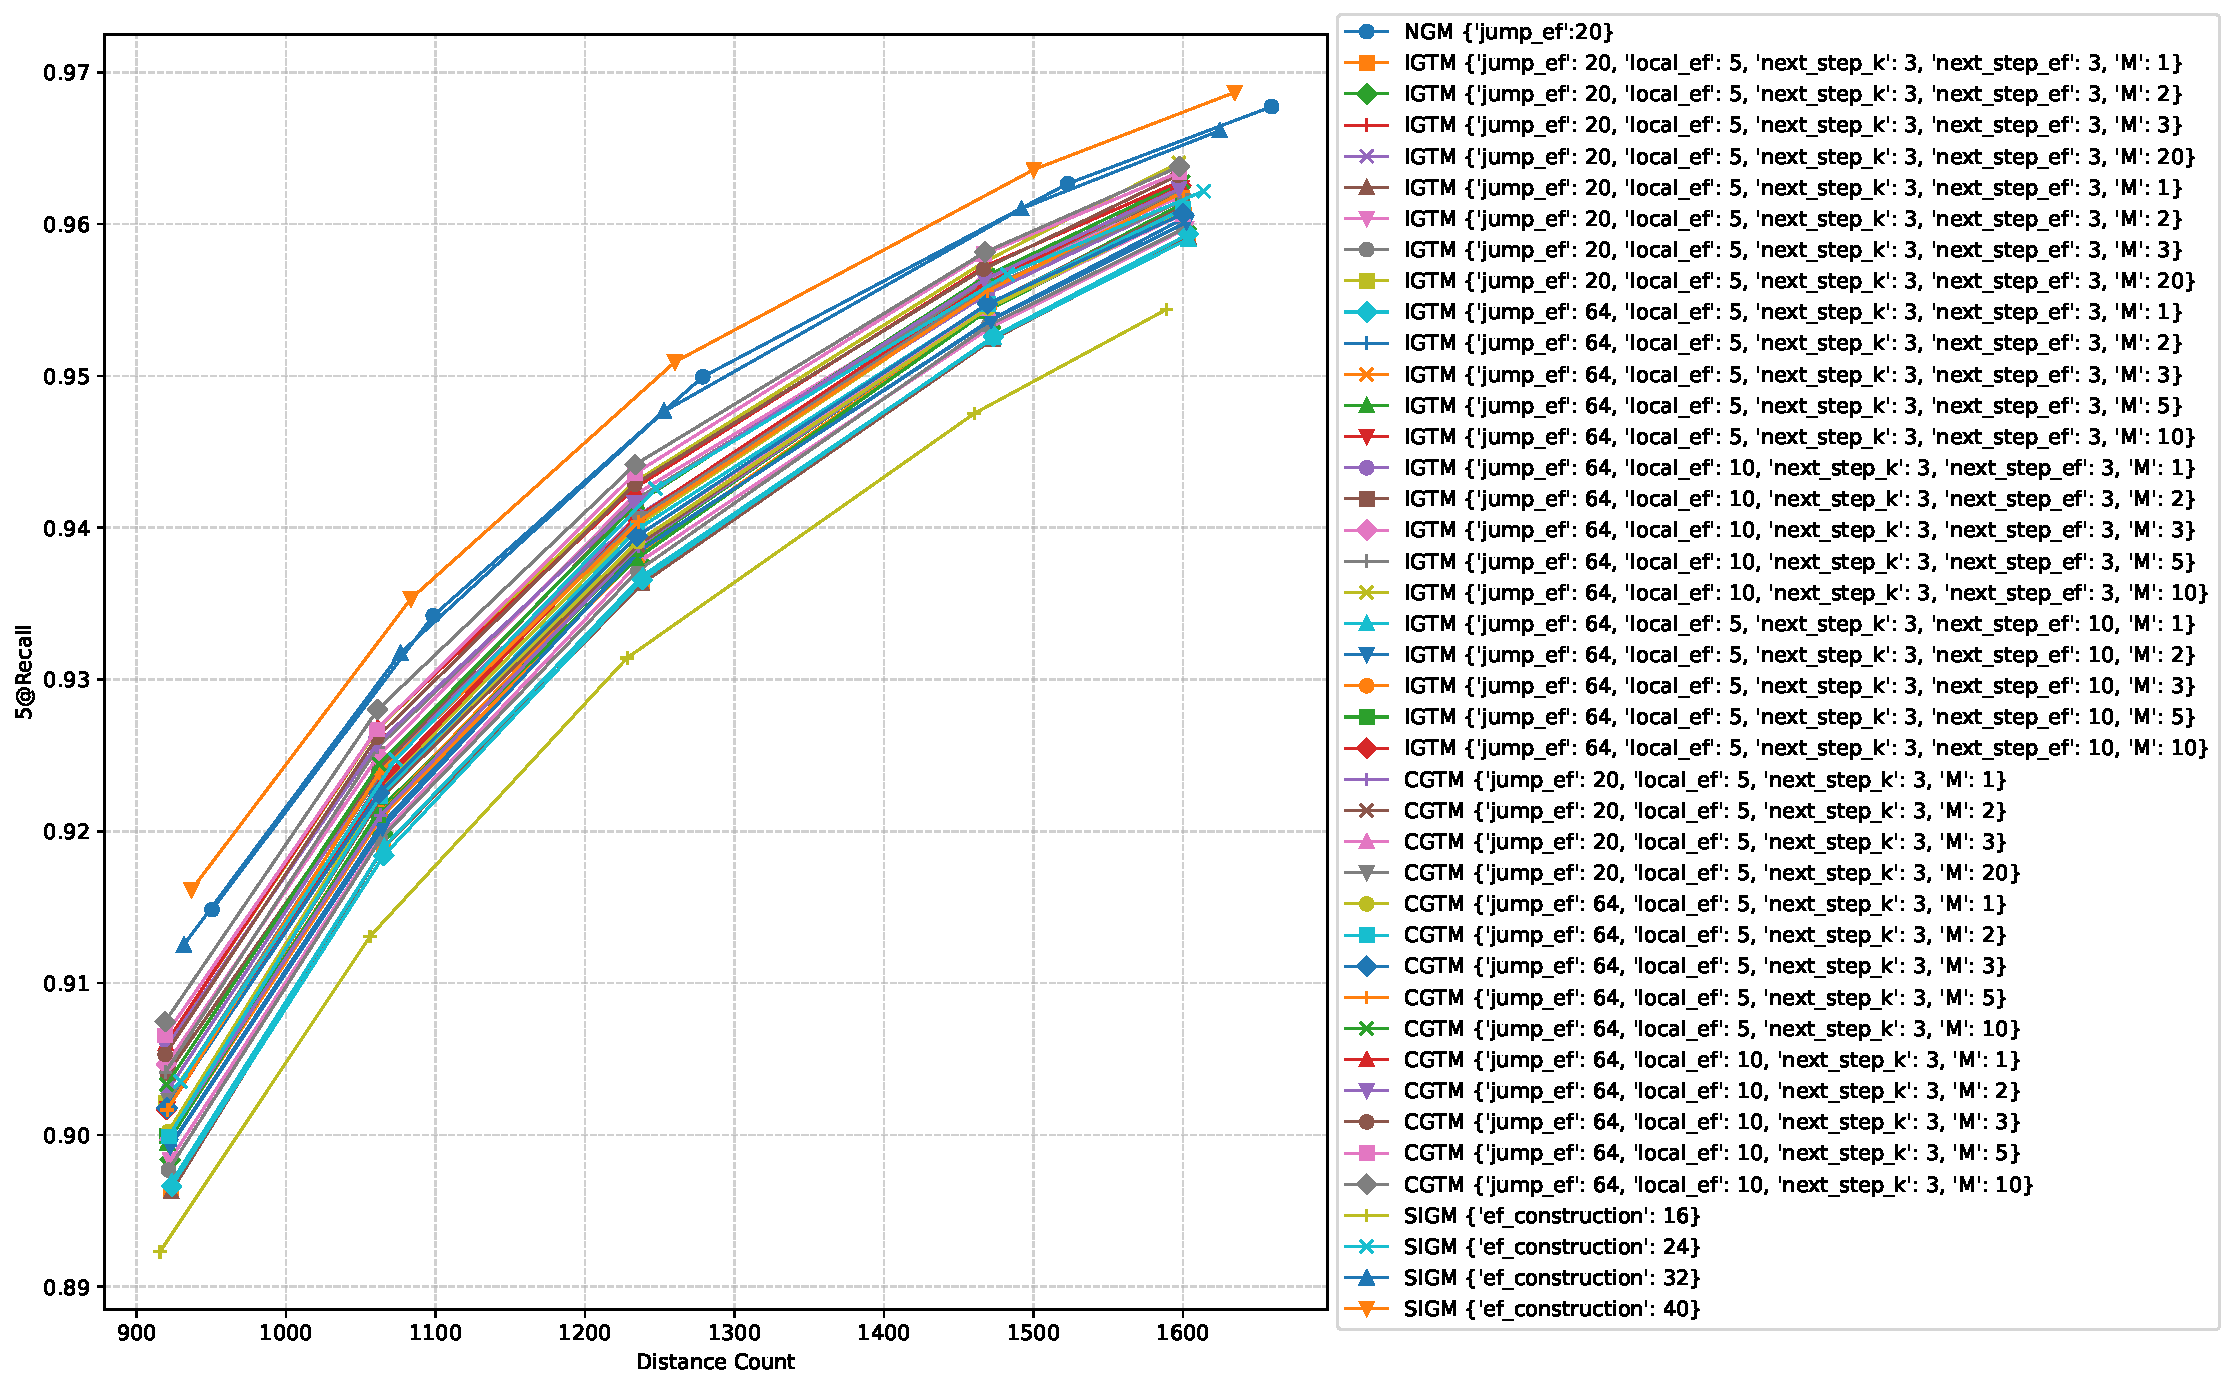
\includegraphics[width=1.\linewidth]{figs/recall_vs_distance_count.pdf}
  \caption{Полнота поиска относительно количества вычислений расстояний на этапе поиска для окончательных объединенных графов}
\label{fig:fig}
\end{figure}

Эти результаты демонстрируют практическую пользу включения приближенного поиска в процесс объединения, позволяя эффективно уплотнять индекс без значительного ухудшения качества поиска.

\begin{figure}
  \centering
  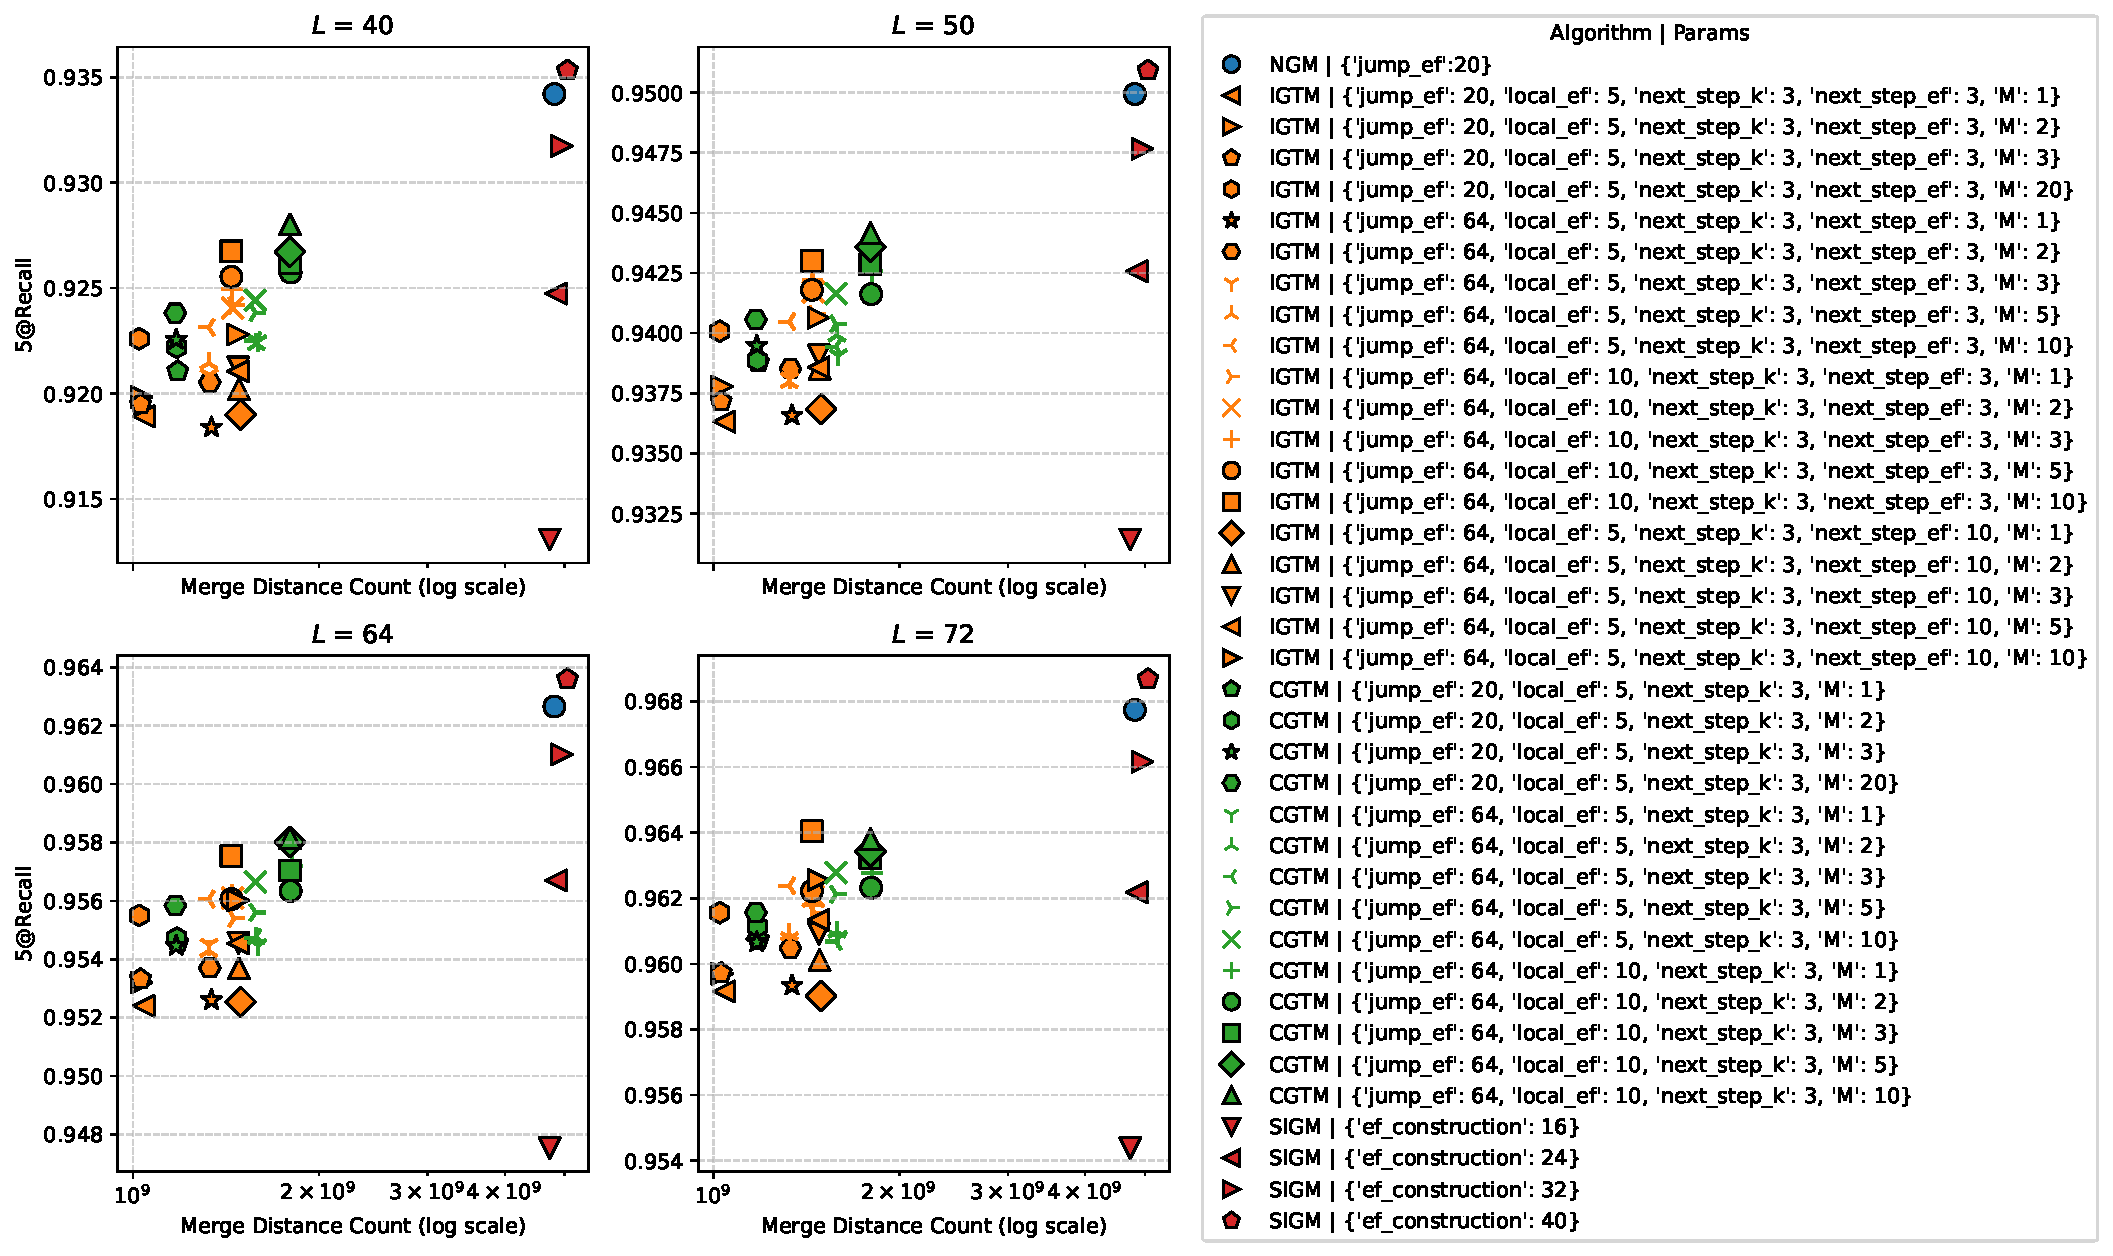
\includegraphics[width=1.\linewidth]{figs/recall_vs_merge_distance_count.pdf}
  \caption{Полнота окончательного объединенного графа в зависимости от затрат на объединение}
  \label{fig:recall_vs_merge}
\end{figure}

\section{Заключение}

В этой работе мы представили три алгоритма для объединения навигационных графов малого мира: \textsc{NGM} (Алгоритм~\ref{alg:merge_naive}), \textsc{IGTM} (Алгоритм~\ref{alg:IGTM}) и \textsc{CGTM} (Алгоритм~\ref{alg:CGTM}). Каждый алгоритм предлагает различные компромиссы между вычислительной эффективностью и качеством структуры объединенного графа. Наши экспериментальные результаты показывают, что \textsc{IGTM} и \textsc{CGTM} значительно уменьшают количество вычислений расстояний по сравнению с наивным подходом, сохраняя при этом сопоставимую точность поиска.

Алгоритм \textsc{NGM} представляет собой прямолинейный, но вычислительно интенсивный подход, выполняющий исчерпывающие поиски для реконструкции окрестности каждой вершины. \textsc{IGTM} повышает эффективность, используя локальность — последовательно обрабатывая вершины, расположенные близко друг к другу, и повторно используя результаты поиска из \textsc{LocalSearch} (Алгоритм~\ref{alg:local_search}). \textsc{CGTM} дополнительно улучшает этот подход, выбирая вершины из обоих входных графов во время процесса объединения, минимизируя дорогостоящие случайные переходы.

Наша оценка по стандартным эталонным наборам данных ANN показывает, что \textsc{IGTM} сокращает вычисления расстояний на 40-60\% по сравнению с \textsc{NGM}, в то время как \textsc{CGTM} достигает до 70\% сокращения с минимальным влиянием на производительность полноты поиска. Эти преимущества в эффективности делают наши алгоритмы особенно ценными для крупномасштабных приложений, где вычислительные ресурсы ограничены.

\subsection{Будущая работа}

Важным направлением для будущей работы является адаптация предложенных алгоритмов объединения для обработки удаленных вершин. Это позволило бы использовать их в процессах уплотнения, где графы периодически реструктурируются для удаления устаревших записей и поддержания эффективности поиска. Расширяя наши алгоритмы объединения для фильтрации удаленных узлов во время фазы построения окрестности (Алгоритм~\ref{alg:knntrategy} или Алгоритм~\ref{alg:rngstrategy}), они могли бы служить эффективными механизмами уплотнения для развивающихся наборов данных.

Дополнительные области для исследования включают стратегии параллелизации для операции \textsc{HNSW-General-Merge} (Алгоритм~\ref{alg:general_merge}), адаптивный выбор параметров на основе характеристик набора данных и расширения для других структур индексов на основе графов помимо HNSW \cite{hnsw}. Дальнейшая оптимизация стратегий построения окрестностей, специально разработанных для объединенных графов, также может привести к улучшению производительности.

\bibliographystyle{plain}
\bibliography{references}

\end{document}